% Options for packages loaded elsewhere
% Options for packages loaded elsewhere
\PassOptionsToPackage{unicode}{hyperref}
\PassOptionsToPackage{hyphens}{url}
%
\documentclass[
  ignorenonframetext,
  aspectratio=169,
]{beamer}
\newif\ifbibliography
\usepackage{pgfpages}
\setbeamertemplate{caption}[numbered]
\setbeamertemplate{caption label separator}{: }
\setbeamercolor{caption name}{fg=normal text.fg}
\beamertemplatenavigationsymbolsempty
% remove section numbering
\setbeamertemplate{part page}{
  \centering
  \begin{beamercolorbox}[sep=16pt,center]{part title}
    \usebeamerfont{part title}\insertpart\par
  \end{beamercolorbox}
}
\setbeamertemplate{section page}{
  \centering
  \begin{beamercolorbox}[sep=12pt,center]{section title}
    \usebeamerfont{section title}\insertsection\par
  \end{beamercolorbox}
}
\setbeamertemplate{subsection page}{
  \centering
  \begin{beamercolorbox}[sep=8pt,center]{subsection title}
    \usebeamerfont{subsection title}\insertsubsection\par
  \end{beamercolorbox}
}
% Prevent slide breaks in the middle of a paragraph
\widowpenalties 1 10000
\raggedbottom
\AtBeginPart{
  \frame{\partpage}
}
\AtBeginSection{
  \ifbibliography
  \else
    \frame{\sectionpage}
  \fi
}
\AtBeginSubsection{
  \frame{\subsectionpage}
}
\usepackage{iftex}
\ifPDFTeX
  \usepackage[T1]{fontenc}
  \usepackage[utf8]{inputenc}
  \usepackage{textcomp} % provide euro and other symbols
\else % if luatex or xetex
  \usepackage{unicode-math} % this also loads fontspec
  \defaultfontfeatures{Scale=MatchLowercase}
  \defaultfontfeatures[\rmfamily]{Ligatures=TeX,Scale=1}
\fi
\usepackage{lmodern}

\usetheme[]{Boadilla}
\usecolortheme[]{default}
\usefonttheme[]{professionalfonts}
\ifPDFTeX\else
  % xetex/luatex font selection
\fi
% Use upquote if available, for straight quotes in verbatim environments
\IfFileExists{upquote.sty}{\usepackage{upquote}}{}
\IfFileExists{microtype.sty}{% use microtype if available
  \usepackage[]{microtype}
  \UseMicrotypeSet[protrusion]{basicmath} % disable protrusion for tt fonts
}{}
\makeatletter
\@ifundefined{KOMAClassName}{% if non-KOMA class
  \IfFileExists{parskip.sty}{%
    \usepackage{parskip}
  }{% else
    \setlength{\parindent}{0pt}
    \setlength{\parskip}{6pt plus 2pt minus 1pt}}
}{% if KOMA class
  \KOMAoptions{parskip=half}}
\makeatother

\usepackage{color}
\usepackage{fancyvrb}
\newcommand{\VerbBar}{|}
\newcommand{\VERB}{\Verb[commandchars=\\\{\}]}
\DefineVerbatimEnvironment{Highlighting}{Verbatim}{commandchars=\\\{\}}
% Add ',fontsize=\small' for more characters per line
\usepackage{framed}
\definecolor{shadecolor}{RGB}{241,243,245}
\newenvironment{Shaded}{\begin{snugshade}}{\end{snugshade}}
\newcommand{\AlertTok}[1]{\textcolor[rgb]{0.68,0.00,0.00}{#1}}
\newcommand{\AnnotationTok}[1]{\textcolor[rgb]{0.37,0.37,0.37}{#1}}
\newcommand{\AttributeTok}[1]{\textcolor[rgb]{0.40,0.45,0.13}{#1}}
\newcommand{\BaseNTok}[1]{\textcolor[rgb]{0.68,0.00,0.00}{#1}}
\newcommand{\BuiltInTok}[1]{\textcolor[rgb]{0.00,0.23,0.31}{#1}}
\newcommand{\CharTok}[1]{\textcolor[rgb]{0.13,0.47,0.30}{#1}}
\newcommand{\CommentTok}[1]{\textcolor[rgb]{0.37,0.37,0.37}{#1}}
\newcommand{\CommentVarTok}[1]{\textcolor[rgb]{0.37,0.37,0.37}{\textit{#1}}}
\newcommand{\ConstantTok}[1]{\textcolor[rgb]{0.56,0.35,0.01}{#1}}
\newcommand{\ControlFlowTok}[1]{\textcolor[rgb]{0.00,0.23,0.31}{\textbf{#1}}}
\newcommand{\DataTypeTok}[1]{\textcolor[rgb]{0.68,0.00,0.00}{#1}}
\newcommand{\DecValTok}[1]{\textcolor[rgb]{0.68,0.00,0.00}{#1}}
\newcommand{\DocumentationTok}[1]{\textcolor[rgb]{0.37,0.37,0.37}{\textit{#1}}}
\newcommand{\ErrorTok}[1]{\textcolor[rgb]{0.68,0.00,0.00}{#1}}
\newcommand{\ExtensionTok}[1]{\textcolor[rgb]{0.00,0.23,0.31}{#1}}
\newcommand{\FloatTok}[1]{\textcolor[rgb]{0.68,0.00,0.00}{#1}}
\newcommand{\FunctionTok}[1]{\textcolor[rgb]{0.28,0.35,0.67}{#1}}
\newcommand{\ImportTok}[1]{\textcolor[rgb]{0.00,0.46,0.62}{#1}}
\newcommand{\InformationTok}[1]{\textcolor[rgb]{0.37,0.37,0.37}{#1}}
\newcommand{\KeywordTok}[1]{\textcolor[rgb]{0.00,0.23,0.31}{\textbf{#1}}}
\newcommand{\NormalTok}[1]{\textcolor[rgb]{0.00,0.23,0.31}{#1}}
\newcommand{\OperatorTok}[1]{\textcolor[rgb]{0.37,0.37,0.37}{#1}}
\newcommand{\OtherTok}[1]{\textcolor[rgb]{0.00,0.23,0.31}{#1}}
\newcommand{\PreprocessorTok}[1]{\textcolor[rgb]{0.68,0.00,0.00}{#1}}
\newcommand{\RegionMarkerTok}[1]{\textcolor[rgb]{0.00,0.23,0.31}{#1}}
\newcommand{\SpecialCharTok}[1]{\textcolor[rgb]{0.37,0.37,0.37}{#1}}
\newcommand{\SpecialStringTok}[1]{\textcolor[rgb]{0.13,0.47,0.30}{#1}}
\newcommand{\StringTok}[1]{\textcolor[rgb]{0.13,0.47,0.30}{#1}}
\newcommand{\VariableTok}[1]{\textcolor[rgb]{0.07,0.07,0.07}{#1}}
\newcommand{\VerbatimStringTok}[1]{\textcolor[rgb]{0.13,0.47,0.30}{#1}}
\newcommand{\WarningTok}[1]{\textcolor[rgb]{0.37,0.37,0.37}{\textit{#1}}}

\usepackage{longtable,booktabs,array}
\newcounter{none} % for unnumbered tables
\usepackage{calc} % for calculating minipage widths
\usepackage{caption}
% Make caption package work with longtable
\makeatletter
\def\fnum@table{\tablename~\thetable}
\makeatother
\usepackage{graphicx}
\makeatletter
\newsavebox\pandoc@box
\newcommand*\pandocbounded[1]{% scales image to fit in text height/width
  \sbox\pandoc@box{#1}%
  \Gscale@div\@tempa{\textheight}{\dimexpr\ht\pandoc@box+\dp\pandoc@box\relax}%
  \Gscale@div\@tempb{\linewidth}{\wd\pandoc@box}%
  \ifdim\@tempb\p@<\@tempa\p@\let\@tempa\@tempb\fi% select the smaller of both
  \ifdim\@tempa\p@<\p@\scalebox{\@tempa}{\usebox\pandoc@box}%
  \else\usebox{\pandoc@box}%
  \fi%
}
% Set default figure placement to htbp
\def\fps@figure{htbp}
\makeatother





\setlength{\emergencystretch}{3em} % prevent overfull lines

\providecommand{\tightlist}{%
  \setlength{\itemsep}{0pt}\setlength{\parskip}{0pt}}



 


\makeatletter
\@ifpackageloaded{tcolorbox}{}{\usepackage[skins,breakable]{tcolorbox}}
\@ifpackageloaded{fontawesome5}{}{\usepackage{fontawesome5}}
\definecolor{quarto-callout-color}{HTML}{909090}
\definecolor{quarto-callout-note-color}{HTML}{0758E5}
\definecolor{quarto-callout-important-color}{HTML}{CC1914}
\definecolor{quarto-callout-warning-color}{HTML}{EB9113}
\definecolor{quarto-callout-tip-color}{HTML}{00A047}
\definecolor{quarto-callout-caution-color}{HTML}{FC5300}
\definecolor{quarto-callout-color-frame}{HTML}{acacac}
\definecolor{quarto-callout-note-color-frame}{HTML}{4582ec}
\definecolor{quarto-callout-important-color-frame}{HTML}{d9534f}
\definecolor{quarto-callout-warning-color-frame}{HTML}{f0ad4e}
\definecolor{quarto-callout-tip-color-frame}{HTML}{02b875}
\definecolor{quarto-callout-caution-color-frame}{HTML}{fd7e14}
\makeatother
\makeatletter
\@ifpackageloaded{caption}{}{\usepackage{caption}}
\AtBeginDocument{%
\ifdefined\contentsname
  \renewcommand*\contentsname{Table of contents}
\else
  \newcommand\contentsname{Table of contents}
\fi
\ifdefined\listfigurename
  \renewcommand*\listfigurename{List of Figures}
\else
  \newcommand\listfigurename{List of Figures}
\fi
\ifdefined\listtablename
  \renewcommand*\listtablename{List of Tables}
\else
  \newcommand\listtablename{List of Tables}
\fi
\ifdefined\figurename
  \renewcommand*\figurename{Figure}
\else
  \newcommand\figurename{Figure}
\fi
\ifdefined\tablename
  \renewcommand*\tablename{Table}
\else
  \newcommand\tablename{Table}
\fi
}
\@ifpackageloaded{float}{}{\usepackage{float}}
\floatstyle{ruled}
\@ifundefined{c@chapter}{\newfloat{codelisting}{h}{lop}}{\newfloat{codelisting}{h}{lop}[chapter]}
\floatname{codelisting}{Listing}
\newcommand*\listoflistings{\listof{codelisting}{List of Listings}}
\makeatother
\makeatletter
\makeatother
\makeatletter
\@ifpackageloaded{caption}{}{\usepackage{caption}}
\@ifpackageloaded{subcaption}{}{\usepackage{subcaption}}
\makeatother

\usepackage{bookmark}
\IfFileExists{xurl.sty}{\usepackage{xurl}}{} % add URL line breaks if available
\urlstyle{same}
\hypersetup{
  pdftitle={Chapter 3: Risk Models},
  hidelinks,
  pdfcreator={LaTeX via pandoc}}


\title{\texorpdfstring{Chapter 3: Risk Models}{Chapter 3: Risk Models}}
\author{}
\date{}

\begin{document}
\frame{\titlepage}


\section{Risk Models}\label{risk-models}

\begin{frame}{Short-Term Risk Models}
\protect\phantomsection\label{short-term-risk-models}
Consider an insurance portfolio over a fixed time interval, such as one
year.

The total amount paid in claims is uncertain because of two sources of
randomness:

\begin{enumerate}
\tightlist
\item
  \textbf{Claim frequency:} how many claims occur.
\item
  \textbf{Claim severity:} how much each claim costs.
\end{enumerate}

For example, a motor portfolio may produce 800 claims in one year and
950 in another. The individual claim amounts can also vary
substantially.

The collective risk model combines these two sources of uncertainty into
a model for the \textbf{aggregate claim amount}.

\begin{tcolorbox}[enhanced jigsaw, arc=.35mm, bottomrule=.15mm, bottomtitle=1mm, breakable, colback=white, colbacktitle=quarto-callout-note-color!10!white, colframe=quarto-callout-note-color-frame, coltitle=black, left=2mm, leftrule=.75mm, opacityback=0, opacitybacktitle=0.6, rightrule=.15mm, title=\textcolor{quarto-callout-note-color}{\faInfo}\hspace{0.5em}{Key idea}, titlerule=0mm, toprule=.15mm, toptitle=1mm]

\textbf{Frequency + severity \(\longrightarrow\) aggregate claims}

\end{tcolorbox}
\end{frame}

\begin{frame}{Frequency and Severity}
\protect\phantomsection\label{frequency-and-severity}
Define the following random variables:

\begin{itemize}
\tightlist
\item
  \(N\): number of claims during the fixed time interval;
\item
  \(X_i\): amount of the \(i\)th claim;
\item
  \(S\): total amount of claims.
\end{itemize}

The claim frequency is a discrete random variable,

\[
N\in\{0,1,2,\ldots\}.
\]

The claim severities \(X_1,X_2,\ldots\) describe the amounts of
individual claims.

For example, \(N\) may have a Poisson distribution, while \(X_i\) may
have a Gamma, Lognormal, or Pareto distribution.
\end{frame}

\begin{frame}{Aggregate Claim Amount}
\protect\phantomsection\label{aggregate-claim-amount}
If exactly \(n\) claims occur, the total claim amount is

\[
S=X_1+\cdots+X_n=\sum_{i=1}^{n}X_i.
\]

But the number of claims is itself random. Therefore,

\[
\boxed{S=\sum_{i=1}^{N}X_i}.
\]

The random variable \(S\) is called the \textbf{aggregate loss},
\textbf{aggregate claim amount}, or \textbf{total claim amount}.

The number of terms in the sum is random because \(N\) is random.
\end{frame}

\begin{frame}{Collective Risk Model Visual Guide}
\protect\phantomsection\label{collective-risk-model-visual-guide}
\begin{center}
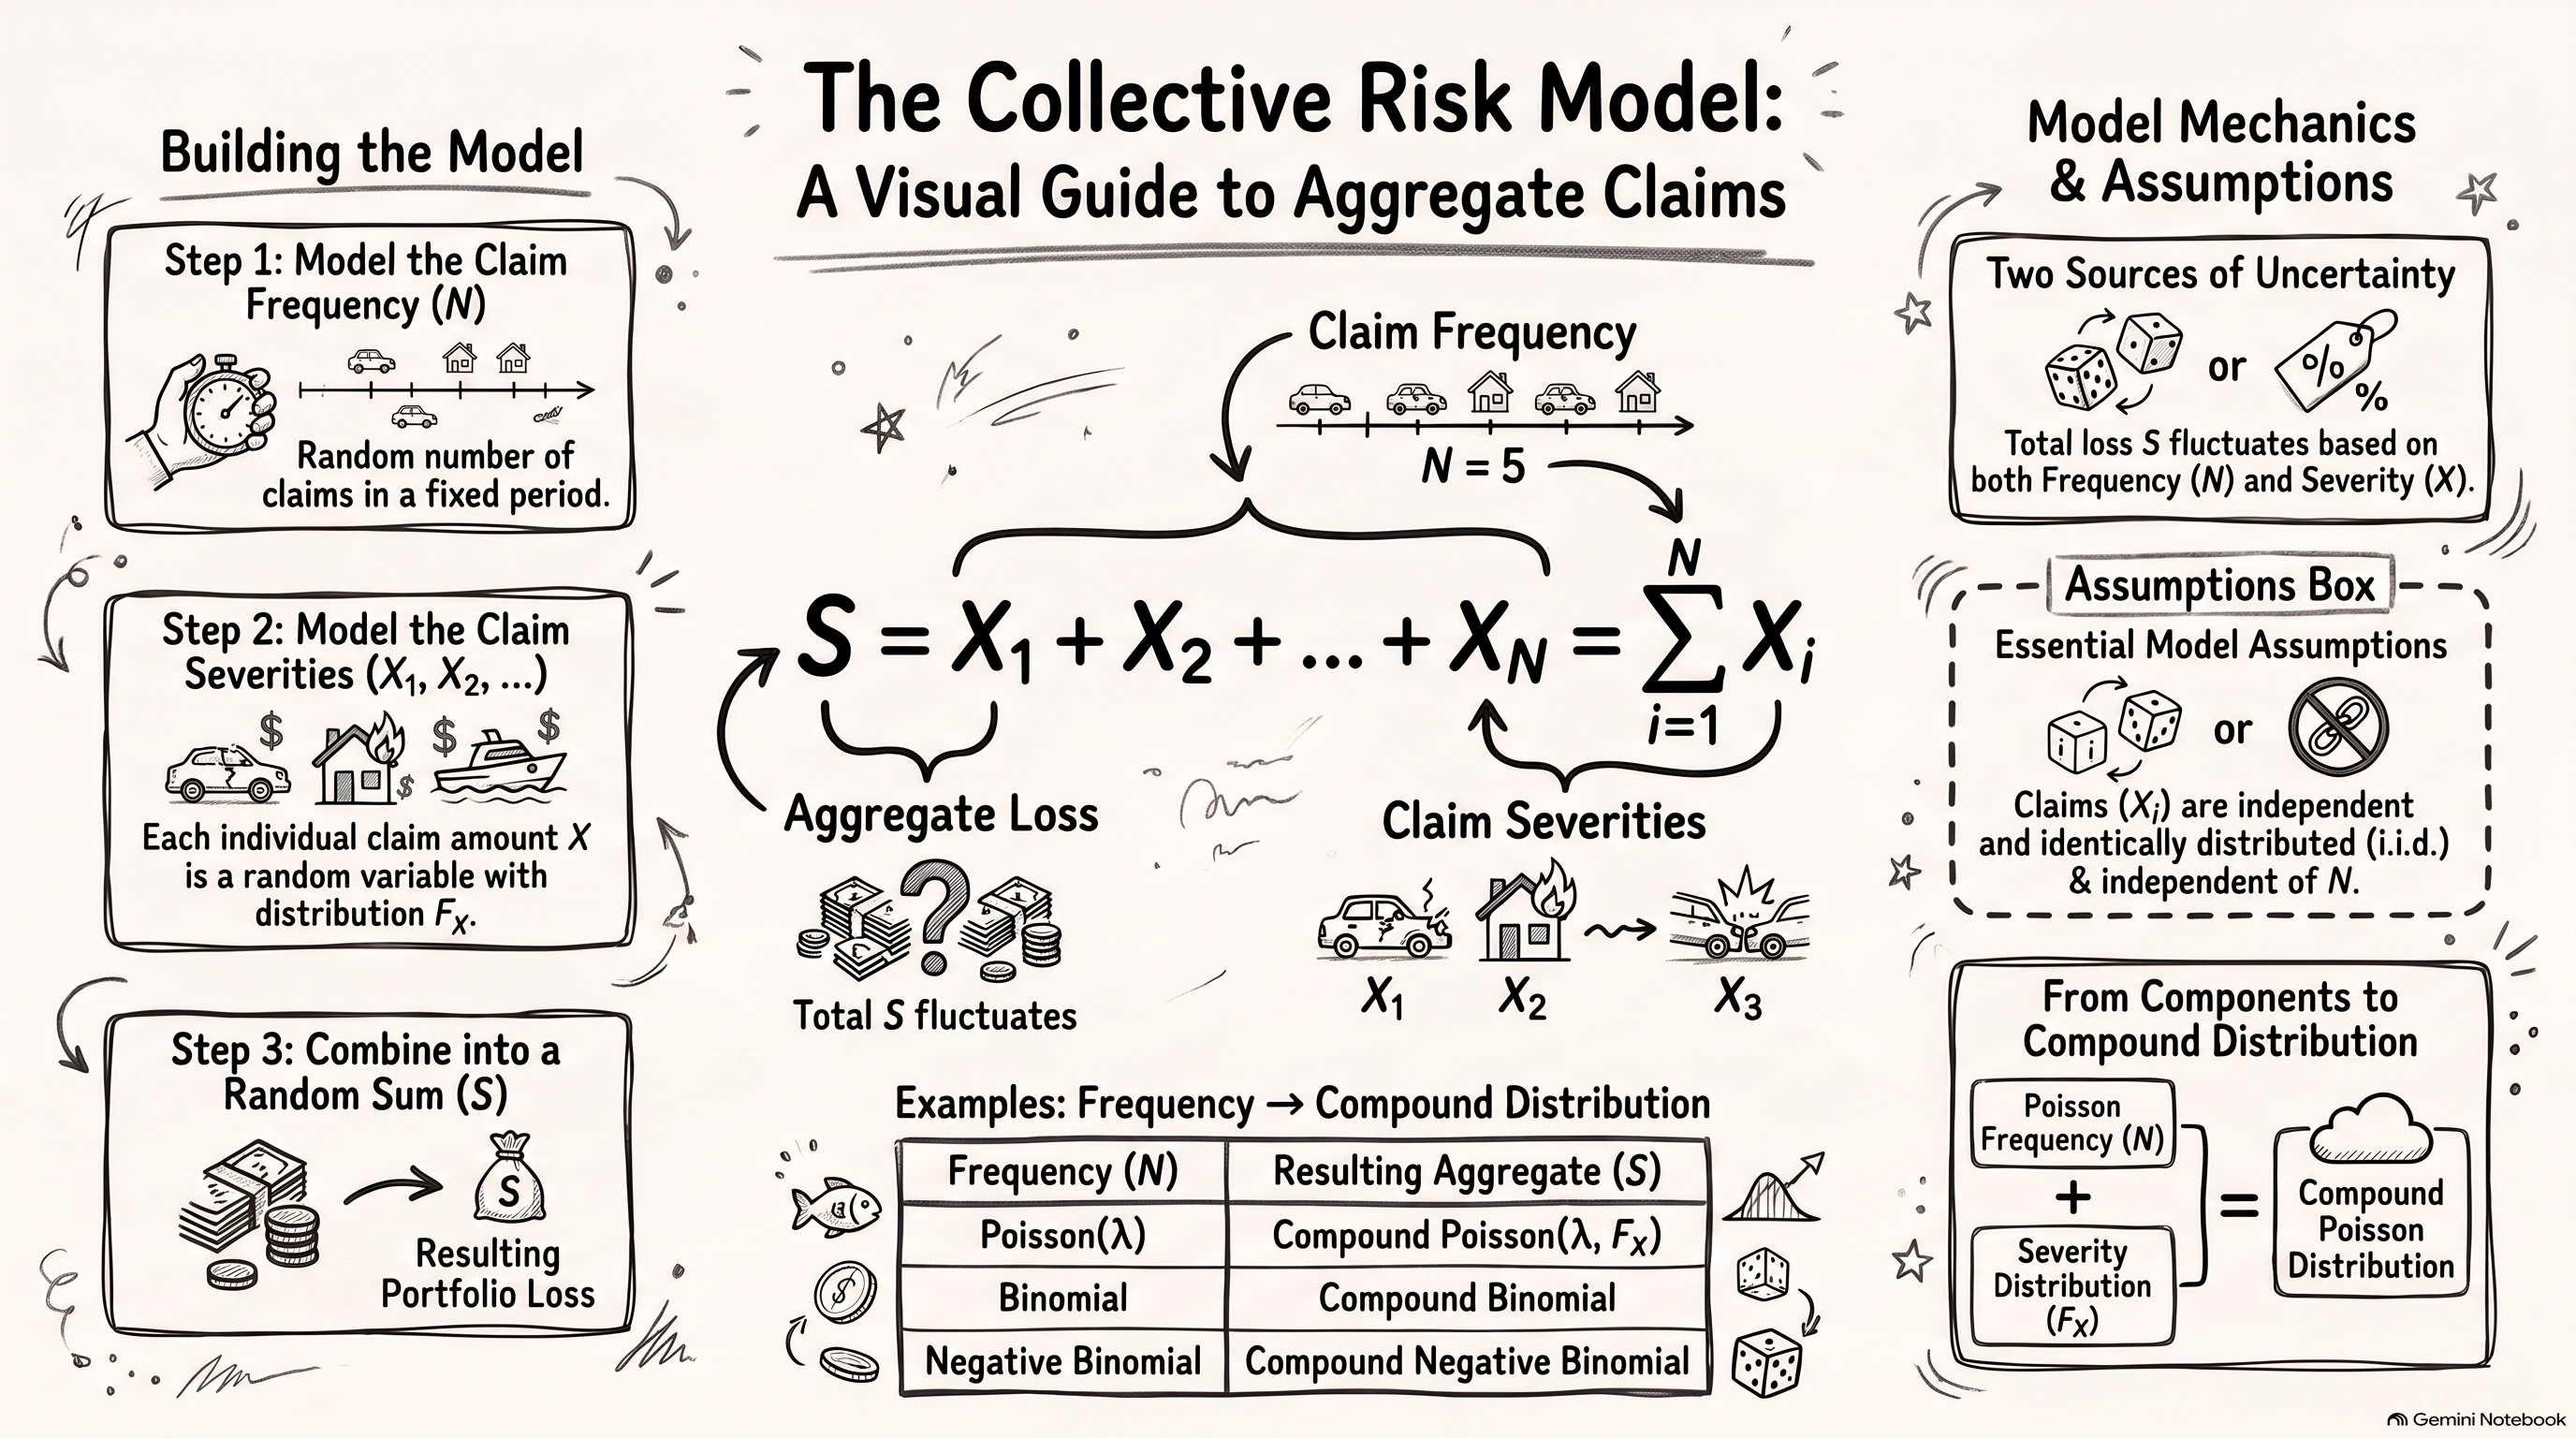
\includegraphics[width=0.8\linewidth,height=\textheight,keepaspectratio]{../figures/Collective_Risk_Model_Visual_Guide.png}
\end{center}
\end{frame}

\begin{frame}{Why Is \(S\) a Random Sum?}
\protect\phantomsection\label{why-is-s-a-random-sum}
The definition

\[
S=\sum_{i=1}^{N}X_i
\]

covers different numbers of claims:

\[
\begin{aligned}
N=0 &\Rightarrow S=0, &
N=1 &\Rightarrow S=X_1,\\
N=2 &\Rightarrow S=X_1+X_2, &
N=n &\Rightarrow S=\sum_{i=1}^{n}X_i.
\end{aligned}
\]

Thus, the collective risk model is a \textbf{random sum model}. The
aggregate loss depends on both the \textbf{number of claims} and their
\textbf{sizes}.
\end{frame}

\begin{frame}{Assumptions of the Collective Risk Model}
\protect\phantomsection\label{assumptions-of-the-collective-risk-model}
The standard collective risk model assumes:

\begin{enumerate}
\item
  The claim severities are independent and identically distributed:

  \[
  X_1,X_2,\ldots \overset{\mathrm{iid}}{\sim} F_X.
  \]
\item
  The claim frequency is independent of all claim severities:

  \[
  N\perp\!\!\!\perp (X_1,X_2,\ldots).
  \]
\end{enumerate}

The first assumption gives all claims the same distribution and makes
different claim amounts independent.

The second assumption means that the number of claims provides no
information about their individual sizes.
\end{frame}

\begin{frame}{Interpretation of the Assumptions}
\protect\phantomsection\label{interpretation-of-the-assumptions}
These assumptions make the aggregate loss mathematically tractable.

In practice, they may not always hold.

For example:

\begin{itemize}
\tightlist
\item
  claim frequency and severity may be dependent;
\item
  claims from the same event may be dependent;
\item
  different types of claims may have different severity distributions.
\end{itemize}

The assumptions are therefore a \textbf{starting model} rather than a
statement that all insurance portfolios behave exactly this way.

\begin{tcolorbox}[enhanced jigsaw, arc=.35mm, bottomrule=.15mm, bottomtitle=1mm, breakable, colback=white, colbacktitle=quarto-callout-warning-color!10!white, colframe=quarto-callout-warning-color-frame, coltitle=black, left=2mm, leftrule=.75mm, opacityback=0, opacitybacktitle=0.6, rightrule=.15mm, title=\textcolor{quarto-callout-warning-color}{\faExclamationTriangle}\hspace{0.5em}{Modelling assumptions}, titlerule=0mm, toprule=.15mm, toptitle=1mm]

\[
\boxed{
X_1,X_2,\ldots\text{ are iid},
\qquad
N\text{ is independent of }X_1,X_2,\ldots
}
\]

Always check whether these assumptions are reasonable for the
application.

\end{tcolorbox}
\end{frame}

\begin{frame}{From Collective Risk Model to Compound Distribution}
\protect\phantomsection\label{from-collective-risk-model-to-compound-distribution}
Under the standard assumptions, \(S=\sum_{i=1}^{N}X_i\)

has a \textbf{compound distribution}.

The model can be viewed as two probability models combined:

\[
\boxed{
\text{Frequency model}
+
\text{Severity model}
\longrightarrow
\text{Aggregate loss model}
}
\]

The distribution chosen for \(N\) determines the type of compound
distribution.

{\def\LTcaptype{none} % do not increment counter
\begin{longtable}[]{@{}ll@{}}
\toprule\noalign{}
Frequency distribution & Aggregate distribution \\
\midrule\noalign{}
\endhead
Binomial & Compound Binomial \\
Poisson & Compound Poisson \\
Negative binomial & Compound Negative Binomial \\
\bottomrule\noalign{}
\end{longtable}
}
\end{frame}

\begin{frame}{Why Study the Collective Risk Model?}
\protect\phantomsection\label{why-study-the-collective-risk-model}
The distribution of

\[
S=\sum_{i=1}^{N}X_i
\]

can, in principle, be obtained using convolution methods.

However, compound distributions generally do not have simple closed-form
distributions.

For this reason, we focus on quantities that can be derived more easily,
particularly:

\begin{itemize}
\tightlist
\item
  \(E[S]\), the expected aggregate loss;
\item
  \(\operatorname{Var}(S)\), the variance of aggregate loss;
\item
  important special compound distributions.
\end{itemize}

These results provide useful measures of the expected cost and
variability of an insurance portfolio.
\end{frame}

\begin{frame}{Actuarial Applications}
\protect\phantomsection\label{actuarial-applications}
Once the aggregate loss model has been specified, it can be used to
study:

\begin{itemize}
\tightlist
\item
  expected total claims; variability of total claims;
\item
  probabilities such as \(\Pr(S>x)\); reinsurance arrangements;
\item
  premium calculations; capital and risk measures.
\end{itemize}

The collective risk model provides a common framework for combining
claim frequency and claim severity.

\begin{tcolorbox}[enhanced jigsaw, arc=.35mm, bottomrule=.15mm, bottomtitle=1mm, breakable, colback=white, colbacktitle=quarto-callout-note-color!10!white, colframe=quarto-callout-note-color-frame, coltitle=black, left=2mm, leftrule=.75mm, opacityback=0, opacitybacktitle=0.6, rightrule=.15mm, title=\textcolor{quarto-callout-note-color}{\faInfo}\hspace{0.5em}{Key idea}, titlerule=0mm, toprule=.15mm, toptitle=1mm]

The central model is

\[
\boxed{S=\sum_{i=1}^{N}X_i}.
\]

The next step is to determine the \textbf{mean and variance of this
random sum}.

\end{tcolorbox}
\end{frame}

\section{Conditional Expectation and
Variance}\label{conditional-expectation-and-variance}

\begin{frame}{Conditional Expectation and Variance Formulas}
\protect\phantomsection\label{conditional-expectation-and-variance-formulas}
Conditional expectation and variance allow us to analyse a random
variable by first conditioning on another random variable.

The \textbf{law of total expectation} is

\[
\boxed{E[E[X\mid Y]]=E[X]}.
\]

The \textbf{law of total variance} is

\[
\boxed{
\operatorname{Var}(X)
=
E[\operatorname{Var}(X\mid Y)]
+
\operatorname{Var}(E[X\mid Y])
}.
\]

These formulas will be used to analyse the aggregate loss

\[
S=\sum_{i=1}^{N}X_i.
\]
\end{frame}

\begin{frame}{Conditional Variance}
\protect\phantomsection\label{conditional-variance}
The conditional variance of \(X\) given \(Y\) is

\[
\operatorname{Var}(X\mid Y)
=
E\left[(X-E[X\mid Y])^2\mid Y\right].
\]

An equivalent expression is

\[
\boxed{
\operatorname{Var}(X\mid Y)
=
E[X^2\mid Y]-(E[X\mid Y])^2
}.
\]

The law of total variance then gives

\[
\operatorname{Var}(X)
=
\underbrace{E[\operatorname{Var}(X\mid Y)]}_{\text{variation within groups}}
+
\underbrace{\operatorname{Var}(E[X\mid Y])}_{\text{variation between groups}}.
\]
\end{frame}

\begin{frame}{Conditional Expectation and Variance Formulas}
\protect\phantomsection\label{conditional-expectation-and-variance-formulas-1}
\begin{center}
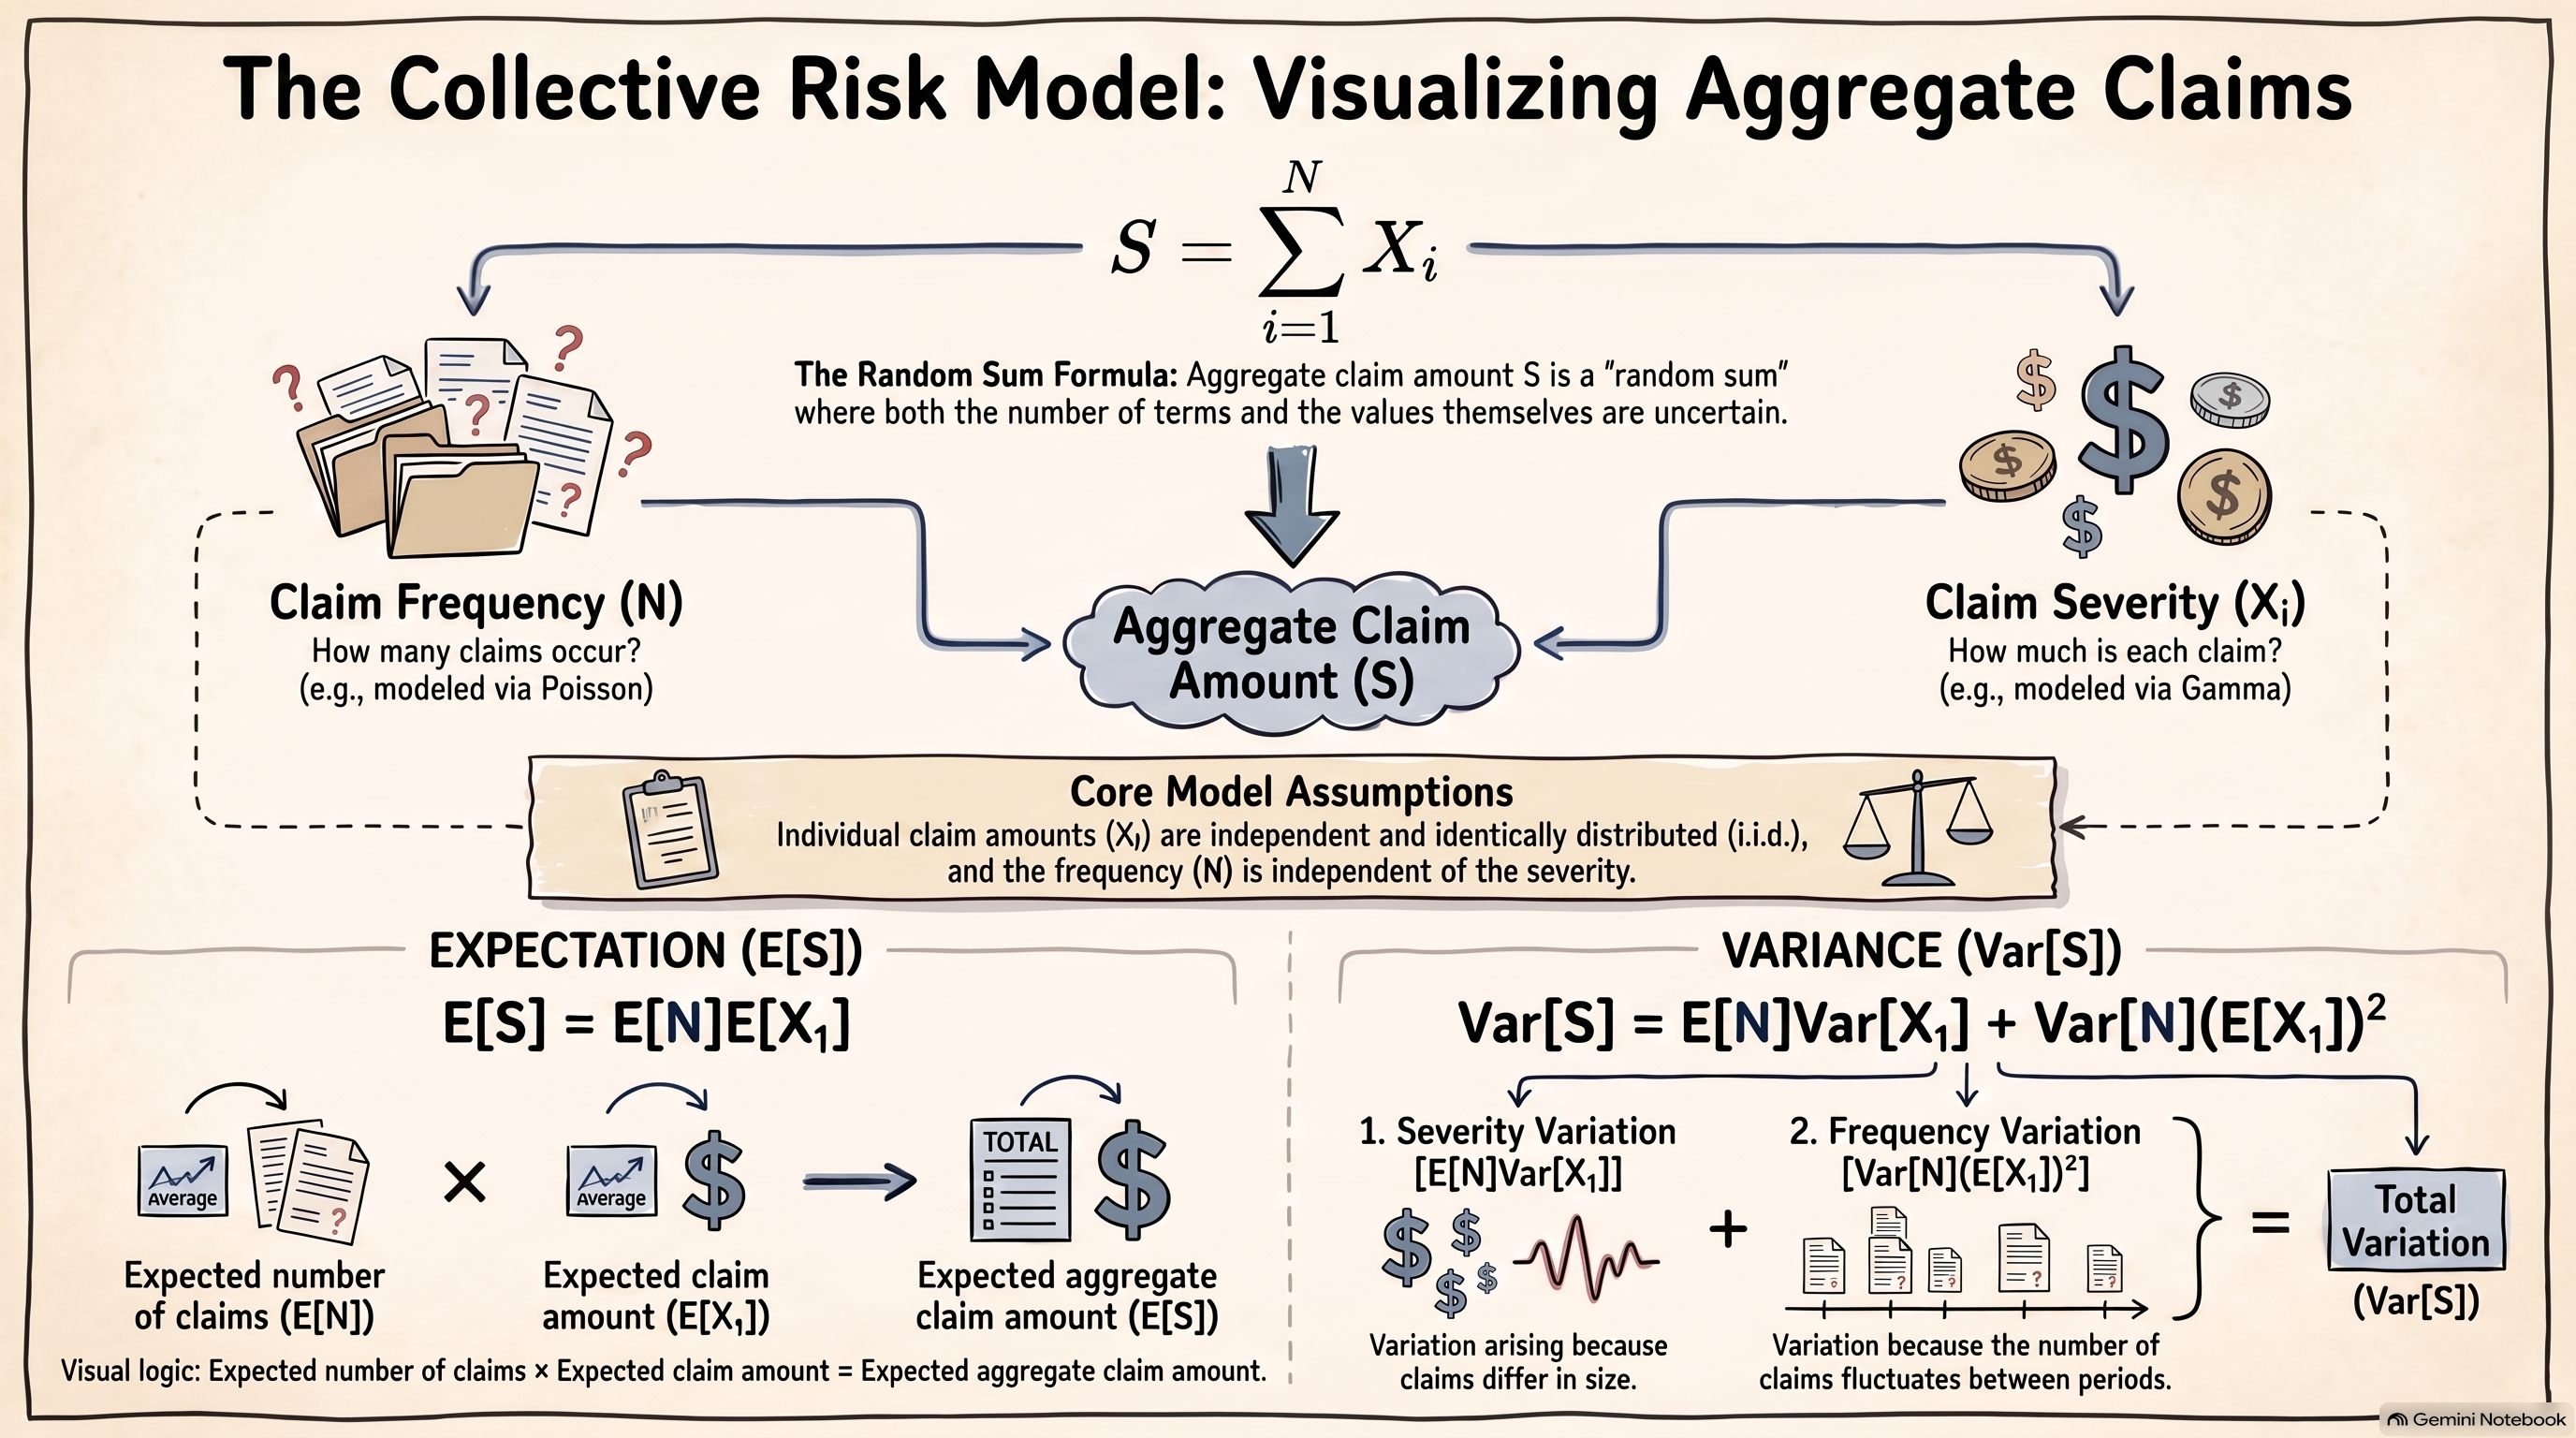
\includegraphics[width=0.8\linewidth,height=\textheight,keepaspectratio]{../figures/The_Collective_Risk_Model_Overview.png}
\end{center}
\end{frame}

\begin{frame}{Example: Conditional Claim Amounts}
\protect\phantomsection\label{example-conditional-claim-amounts}
An insurer classifies policyholders into three risk groups:

\[
Y\in\{L,M,H\},
\qquad
P(L)=P(M)=P(H)=\frac13.
\]

Conditional on the risk group, two claim amounts are equally likely.

{\def\LTcaptype{none} % do not increment counter
\begin{longtable}[]{@{}lr@{}}
\toprule\noalign{}
Risk group & Claim amounts (THB) \\
\midrule\noalign{}
\endhead
Low (\(L\)) & \(1,2\) \\
Medium (\(M\)) & \(1,5\) \\
High (\(H\)) & \(1,10\) \\
\bottomrule\noalign{}
\end{longtable}
}

Let \(X\) denote the claim amount of a randomly selected policyholder.
\end{frame}

\begin{frame}{Example: Conditional Claim Amounts}
\protect\phantomsection\label{example-conditional-claim-amounts-1}
\textbf{Questions}

\begin{enumerate}
\tightlist
\item
  Find the distribution of \(X\).
\item
  Find \(E[X]\) and \(\operatorname{Var}(X)\).
\item
  Verify the results using conditional expectation and variance.
\end{enumerate}
\end{frame}

\begin{frame}{Distribution of the Claim Amount}
\protect\phantomsection\label{distribution-of-the-claim-amount}
The possible claim amounts are

\[
X\in\{1,2,5,10\}.
\]

For example,

\[
\begin{aligned}
P(X=1)
&=\sum_{y\in\{L,M,H\}}P(X=1\mid Y=y)P(Y=y)\\
&=\frac12\left(\frac13+\frac13+\frac13\right)
=\frac12.
\end{aligned}
\]

Similarly,

\[
P(X=2)=P(X=5)=P(X=10)=\frac16.
\]
\end{frame}

\begin{frame}{Distribution of the Claim Amount}
\protect\phantomsection\label{distribution-of-the-claim-amount-1}
Therefore, the probability distribution of \(X\) is

{\def\LTcaptype{none} % do not increment counter
\begin{longtable}[]{@{}lrrrr@{}}
\toprule\noalign{}
\(x\) & \(1\) & \(2\) & \(5\) & \(10\) \\
\midrule\noalign{}
\endhead
\(P(X=x)\) & \(\frac12\) & \(\frac16\) & \(\frac16\) & \(\frac16\) \\
\bottomrule\noalign{}
\end{longtable}
}
\end{frame}

\begin{frame}{Direct Calculation of the Mean}
\protect\phantomsection\label{direct-calculation-of-the-mean}
Using the distribution of \(X\),

\[
\begin{aligned}
E[X]
&=1\left(\frac12\right)
+2\left(\frac16\right)
+5\left(\frac16\right)
+10\left(\frac16\right)\\
&=\frac{10}{3}.
\end{aligned}
\]

Thus,

\[
\boxed{E[X]=\frac{10}{3}}.
\]
\end{frame}

\begin{frame}{Direct Calculation of the Variance}
\protect\phantomsection\label{direct-calculation-of-the-variance}
First calculate the second moment:

\[
\begin{aligned}
E[X^2]
&=1^2\left(\frac12\right)
+2^2\left(\frac16\right)
+5^2\left(\frac16\right)
+10^2\left(\frac16\right)\\
&=22.
\end{aligned}
\]

Hence,

\[
\begin{aligned}
\operatorname{Var}(X)
&=E[X^2]-(E[X])^2\\
&=22-\left(\frac{10}{3}\right)^2\\
&=\frac{98}{9}.
\end{aligned}
\]
\end{frame}

\begin{frame}{Conditional Means}
\protect\phantomsection\label{conditional-means}
Let \(Y\) denote the risk group.

For the three groups,

\[
\begin{aligned}
E[X\mid L]&=\frac{1+2}{2}=\frac32,\\
E[X\mid M]&=\frac{1+5}{2}=3,\\
E[X\mid H]&=\frac{1+10}{2}=\frac{11}{2}.
\end{aligned}
\]

Using the law of total expectation,

\[
\begin{aligned}
E[X]
&=E[E[X\mid Y]]\\
&=\frac13\left(
\frac32+3+\frac{11}{2}
\right)=\frac{10}{3}.
\end{aligned}
\]

This agrees with the direct calculation.
\end{frame}

\begin{frame}{Conditional Variances}
\protect\phantomsection\label{conditional-variances}
For two equally likely values \(a\) and \(b\),

\[
\operatorname{Var}(X)
=
\frac{a^2+b^2}{2}
-\left(\frac{a+b}{2}\right)^2.
\]

Therefore,

\[
\operatorname{Var}(X\mid L)=\frac14,\qquad \operatorname{Var}(X\mid M)=4,\qquad \operatorname{Var}(X\mid H)=\frac{81}{4}.
\]

The average within-group variation is

\[
\begin{aligned}
E[\operatorname{Var}(X\mid Y)]
&=\frac13\left(
\frac14+4+\frac{81}{4}
\right) = \frac{49}{6}.
\end{aligned}
\]
\end{frame}

\begin{frame}{Variation Between Risk Groups}
\protect\phantomsection\label{variation-between-risk-groups}
The conditional means are

\[
\frac32,\qquad 3,\qquad \frac{11}{2},
\]

with overall mean \(\frac{10}{3}\).

Hence,

\[
\begin{aligned}
\operatorname{Var}(E[X\mid Y])
&=\frac13\left[
\left(\frac32-\frac{10}{3}\right)^2
+\left(3-\frac{10}{3}\right)^2
+\left(\frac{11}{2}-\frac{10}{3}\right)^2
\right]\\
&=\frac{49}{18}.
\end{aligned}
\]

This measures the variation in average claim amounts \textbf{between
risk groups}.
\end{frame}

\begin{frame}{Verify the Total Variance}
\protect\phantomsection\label{verify-the-total-variance}
The law of total variance gives

\[
\begin{aligned}
\operatorname{Var}(X)
&=E[\operatorname{Var}(X\mid Y)]
+\operatorname{Var}(E[X\mid Y])\\
&=\frac{49}{6}+\frac{49}{18}=\frac{98}{9}.
\end{aligned}
\]

Thus, the conditional calculation agrees with the direct calculation.

\begin{tcolorbox}[enhanced jigsaw, arc=.35mm, bottomrule=.15mm, bottomtitle=1mm, breakable, colback=white, colbacktitle=quarto-callout-note-color!10!white, colframe=quarto-callout-note-color-frame, coltitle=black, left=2mm, leftrule=.75mm, opacityback=0, opacitybacktitle=0.6, rightrule=.15mm, title=\textcolor{quarto-callout-note-color}{\faInfo}\hspace{0.5em}{Interpretation}, titlerule=0mm, toprule=.15mm, toptitle=1mm]

\[
\boxed{
\operatorname{Var}(X)
=
\underbrace{E[\operatorname{Var}(X\mid Y)]}_{\text{within-group variation}}
+
\underbrace{\operatorname{Var}(E[X\mid Y])}_{\text{between-group variation}}
}
\]

Total uncertainty consists of variation \textbf{within} risk groups and
variation \textbf{between} their average claim amounts.

\end{tcolorbox}
\end{frame}

\begin{frame}{Application to the Collective Risk Model}
\protect\phantomsection\label{application-to-the-collective-risk-model}
Consider the aggregate claim amount

\[
S=\sum_{i=1}^{N}X_i.
\]

Conditioning on the number of claims \(N=n\) gives

\[
S\mid(N=n)=\sum_{i=1}^{n}X_i.
\]

If the claim amounts are iid with

\[
E[X_i]=\mu_X,
\qquad
\operatorname{Var}(X_i)=\sigma_X^2,
\]

then \(\boxed{E[S\mid N=n]=n\mu_X}.\)
\end{frame}

\begin{frame}{Application to the Collective Risk Model}
\protect\phantomsection\label{application-to-the-collective-risk-model-1}
Since the claim amounts are independent,

\[
\boxed{\operatorname{Var}(S\mid N=n)=n\sigma_X^2}.
\]

Thus, conditional on \(N=n\), the aggregate claim amount has

\[
E[S\mid N=n]=n\mu_X,
\qquad
\operatorname{Var}(S\mid N=n)=n\sigma_X^2.
\]

These results provide the starting point for deriving the moments of the
collective risk model.
\end{frame}

\begin{frame}{From Conditional to Unconditional Moments}
\protect\phantomsection\label{from-conditional-to-unconditional-moments}
Using the law of total expectation,

\[
\begin{aligned}
E[S]
&=E[E[S\mid N]]\\
&=E[N\mu_X]\\
&=\mu_XE[N].
\end{aligned}
\]

Using the law of total variance,

\[
\begin{aligned}
\operatorname{Var}(S)
&=E[\operatorname{Var}(S\mid N)]
+\operatorname{Var}(E[S\mid N])\\
&=E[N\sigma_X^2]
+\operatorname{Var}(N\mu_X).
\end{aligned}
\]

Therefore,

\[
\boxed{
\operatorname{Var}(S)
=
\sigma_X^2E[N]
+\mu_X^2\operatorname{Var}(N)
}.
\]
\end{frame}

\section{Moments of the Collective Risk
Model}\label{moments-collective-risk-model}

\begin{frame}{General Setup}
\protect\phantomsection\label{general-setup}
Recall the collective risk model

\[
S=\sum_{i=1}^{N}X_i,
\]

where \(N\) is the number of claims and \(X_i\) is the amount of the
\(i\)th claim.

Assume

\[
X_1,X_2,\ldots \overset{\mathrm{iid}}{\sim} F_X,
\qquad
N\perp\!\!\!\perp (X_1,X_2,\ldots).
\]

We derive the moments of \(S\) by \textbf{conditioning on \(N\)}.

Let

\[
\mu_X=E[X_1],
\qquad
\sigma_X^2=\operatorname{Var}(X_1).
\]
\end{frame}

\begin{frame}{Mean of the Aggregate Loss}
\protect\phantomsection\label{mean-of-the-aggregate-loss}
Conditional on \(N=n\), \(S=\sum_{i=1}^{n}X_i.\)

Therefore,

\[
E[S\mid N=n]
=
\sum_{i=1}^{n}E[X_i]
=
n\mu_X.
\]

Using the law of total expectation,

\[
\begin{aligned}
E[S]
&=E[E[S\mid N]]=E[N\mu_X]=\mu_XE[N].
\end{aligned}
\]

Hence,

\[
\boxed{
E[S]=E[N]E[X_1]
}.
\]
\end{frame}

\begin{frame}{Interpretation of the Mean}
\protect\phantomsection\label{interpretation-of-the-mean}
The result

\[
\boxed{E[S]=E[N]E[X_1]}
\]

has a simple interpretation:

\[
\text{Expected aggregate claims}
=
\text{Expected number of claims}
\times
\text{Expected claim amount}.
\]

For example, if

\[
E[N]=100
\qquad\text{and}\qquad
E[X_1]=5{,}000,
\]

then

\[
E[S]=100(5{,}000)=500{,}000.
\]
\end{frame}

\begin{frame}{Variance of the Aggregate Loss}
\protect\phantomsection\label{variance-of-the-aggregate-loss}
Let

\[
m_1=E[X_1],
\qquad
m_2=E[X_1^2].
\]

Then

\[
\operatorname{Var}(X_1)=m_2-m_1^2.
\]

Conditional on \(N=n\),

\[
\operatorname{Var}(S\mid N=n)
=
n\operatorname{Var}(X_1).
\]

Also,

\[
E[S\mid N=n]=nm_1.
\]
\end{frame}

\begin{frame}{Deriving the Variance}
\protect\phantomsection\label{deriving-the-variance}
By the law of total variance,

\[
\begin{aligned}
\operatorname{Var}(S)
&=E[\operatorname{Var}(S\mid N)]
+\operatorname{Var}(E[S\mid N])\\
&=E[N\operatorname{Var}(X_1)]
+\operatorname{Var}(Nm_1).
\end{aligned}
\]

Since \(m_1\) and \(\operatorname{Var}(X_1)\) are constants,

\[
\boxed{
\operatorname{Var}(S)
=
E[N]\operatorname{Var}(X_1)
+
\operatorname{Var}(N)(E[X_1])^2
}.
\]
\end{frame}

\begin{frame}{Interpretation of the Variance}
\protect\phantomsection\label{interpretation-of-the-variance}
The variance decomposes into two sources:

\[
\boxed{
\operatorname{Var}(S)
=
\underbrace{E[N]\operatorname{Var}(X_1)}
_{\text{claim severity variation}}
+
\underbrace{\operatorname{Var}(N)(E[X_1])^2}
_{\text{claim frequency variation}}
}
\]

\begin{itemize}
\tightlist
\item
  The first term arises from variation in individual claim amounts.
\item
  The second term arises because the number of claims is random.
\end{itemize}

Thus, both \textbf{severity uncertainty} and \textbf{frequency
uncertainty} contribute to aggregate risk.
\end{frame}

\begin{frame}{Third Central Moment}
\protect\phantomsection\label{third-central-moment}
To study skewness, define

\[
\mu_X=E[X_1],
\qquad
\sigma_X^2=\operatorname{Var}(X_1),
\]

and

\[
\mu_{3,X}
=
E[(X_1-\mu_X)^3].
\]

For the claim frequency \(N\), define

\[
\mu_N=E[N],
\qquad
\sigma_N^2=\operatorname{Var}(N),
\]

and

\[
\mu_{3,N}
=
E[(N-\mu_N)^3].
\]
\end{frame}

\begin{frame}{Third Central Moment of \(S\)}
\protect\phantomsection\label{third-central-moment-of-s}
For the random sum

\[
S=\sum_{i=1}^{N}X_i,
\]

the third central moment is

\[
\boxed{
\mu_{3,S}
=
\mu_N\mu_{3,X}
+
3\sigma_N^2\mu_X\sigma_X^2
+
\mu_{3,N}\mu_X^3
}.
\]

The three terms have distinct sources:

\begin{enumerate}
\tightlist
\item
  individual claim severity;
\item
  interaction between frequency and severity variation;
\item
  skewness of the claim frequency.
\end{enumerate}
\end{frame}

\begin{frame}{Coefficient of Skewness}
\protect\phantomsection\label{coefficient-of-skewness}
For a random variable \(X\), the coefficient of skewness is

\[
\gamma_1
=
\frac{E[(X-E[X])^3]}
{\operatorname{Var}(X)^{3/2}}.
\]

Therefore,

\[
\boxed{
\gamma_{1,S}
=
\frac{\mu_{3,S}}
{\operatorname{Var}(S)^{3/2}}
}.
\]

Substituting the collective risk model moments gives

\[
\boxed{
\gamma_{1,S}
=
\frac{
\mu_N\mu_{3,X}
+
3\sigma_N^2\mu_X\sigma_X^2
+
\mu_{3,N}\mu_X^3
}{
\left(
\mu_N\sigma_X^2+\sigma_N^2\mu_X^2
\right)^{3/2}
}
}.
\]
\end{frame}

\begin{frame}{Summary of the First Three Moments}
\protect\phantomsection\label{summary-of-the-first-three-moments}
For \(S=\sum_{i=1}^{N}X_i\), define

\[
\mu_N=E[N],\qquad
\sigma_N^2=\operatorname{Var}(N),\qquad
\mu_{3,N}=E[(N-\mu_N)^3].
\]

and

\[
\mu_X=E[X_1],\qquad
\sigma_X^2=\operatorname{Var}(X_1),\qquad
\mu_{3,X}=E[(X_1-\mu_X)^3].
\]

Then the first moment is

\[
\boxed{E[S]=\mu_N\mu_X}.
\]
\end{frame}

\begin{frame}{Summary of the First Three Moments}
\protect\phantomsection\label{summary-of-the-first-three-moments-1}
The variance is

\[
\boxed{
\operatorname{Var}(S)
=
\mu_N\sigma_X^2+\sigma_N^2\mu_X^2
}.
\]

The third central moment is

\[
\boxed{
\mu_{3,S}
=
\mu_N\mu_{3,X}
+
3\sigma_N^2\mu_X\sigma_X^2
+
\mu_{3,N}\mu_X^3
}.
\]
\end{frame}

\begin{frame}{Reading the Moment Formulas}
\protect\phantomsection\label{reading-the-moment-formulas}
The collective risk model combines two random quantities:

\[
\boxed{
N
\quad\text{and}\quad
X_1,X_2,\ldots
}
\]

The aggregate moments therefore depend on moments of \textbf{both
frequency and severity}.

{\def\LTcaptype{none} % do not increment counter
\begin{longtable}[]{@{}
  >{\raggedright\arraybackslash}p{(\linewidth - 2\tabcolsep) * \real{0.2644}}
  >{\raggedright\arraybackslash}p{(\linewidth - 2\tabcolsep) * \real{0.7356}}@{}}
\toprule\noalign{}
\begin{minipage}[b]{\linewidth}\raggedright
Aggregate quantity
\end{minipage} & \begin{minipage}[b]{\linewidth}\raggedright
Depends on
\end{minipage} \\
\midrule\noalign{}
\endhead
\(E[S]\) & \(E[N]\), \(E[X]\) \\
\(\operatorname{Var}(S)\) & \(E[N]\), \(\operatorname{Var}(N)\),
\(\operatorname{Var}(X)\), \(E[X]\) \\
\(\mu_{3,S}\) & first three moments of \(N\) and \(X\) \\
\bottomrule\noalign{}
\end{longtable}
}

This allows different frequency distributions to be compared while
keeping the same severity model.
\end{frame}

\begin{frame}{Moment Generating Function}
\protect\phantomsection\label{moment-generating-function}
The random-sum representation also gives a general formula for the MGF.

Let

\[
M_X(t)=E[e^{tX_1}],
\qquad
M_N(t)=E[e^{tN}].
\]

Conditional on \(N=n\),

\[
\begin{aligned}
E[e^{tS}\mid N=n]
&=
E\left[
e^{t(X_1+\cdots+X_n)}
\right]\\
&=
\prod_{i=1}^{n}E[e^{tX_i}]\\
&=
\left(M_X(t)\right)^n.
\end{aligned}
\]

The independence of the claim amounts is used here.
\end{frame}

\begin{frame}{Deriving the Aggregate MGF}
\protect\phantomsection\label{deriving-the-aggregate-mgf}
Since

\[
E[e^{tS}\mid N]
=
\left(M_X(t)\right)^N,
\]

the law of total expectation gives

\[
\begin{aligned}
M_S(t)
&=E[e^{tS}]\\
&=E\left[\left(M_X(t)\right)^N\right]\\
&=E\left[
e^{N\log(M_X(t))}
\right].
\end{aligned}
\]

Using the definition of \(M_N\),

\[
\boxed{
M_S(t)
=
M_N\left(\log M_X(t)\right)
}.
\]

This is the general MGF formula for the collective risk model.
\end{frame}

\begin{frame}{Using the Aggregate MGF}
\protect\phantomsection\label{using-the-aggregate-mgf}
The formula

\[
\boxed{
M_S(t)=M_N\left(\log M_X(t)\right)
}
\]

means that the aggregate MGF can be obtained from:

\begin{itemize}
\tightlist
\item
  the MGF of the claim severity, \(M_X(t)\); and
\item
  the MGF of the claim frequency, \(M_N(t)\).
\end{itemize}

Once these two MGFs are known, substitute

\[
t\longmapsto \log M_X(t)
\]

into \(M_N(t)\).

This provides another route to the moments of \(S\).
\end{frame}

\begin{frame}{From General to Special Models}
\protect\phantomsection\label{from-general-to-special-models}
The general results apply to any claim frequency distribution for which
the required moments exist.

Important cases include:

\[
\boxed{
\begin{array}{ccc}
N &\longrightarrow& S\\[2pt]
\text{Binomial}
&\longrightarrow&
\text{Compound Binomial}\\
\text{Poisson}
&\longrightarrow&
\text{Compound Poisson}\\
\text{Negative binomial}
&\longrightarrow&
\text{Compound Negative Binomial}
\end{array}
}
\]

The next section considers these \textbf{special compound distributions}
and their properties.
\end{frame}

\section{Special Compound
Distributions}\label{special-compound-distributions}

\begin{frame}{Compound Poisson Distribution}
\protect\phantomsection\label{compound-poisson-distribution}
Suppose the claim frequency follows a Poisson distribution:

\[
N\sim\operatorname{Poisson}(\lambda).
\]

Assume the claim severities are iid and independent of \(N\):

\[
X_1,X_2,\ldots\overset{\mathrm{iid}}{\sim}F_X.
\]

The aggregate claim amount is

\[
S=\sum_{i=1}^{N}X_i.
\]

Then \(S\) has a \textbf{compound Poisson distribution}, written as
\(\boxed{S\sim\mathcal{CP}(\lambda,F_X)}.\)
\end{frame}

\begin{frame}{Compound Poisson Model}
\protect\phantomsection\label{compound-poisson-model}
The compound Poisson model combines:

\[
\boxed{
\begin{array}{c}
N\sim\operatorname{Poisson}(\lambda)\\
X_i\sim F_X
\end{array}
}
\quad\Longrightarrow\quad
\boxed{
S=\sum_{i=1}^{N}X_i
}
\]

Here,

\begin{itemize}
\tightlist
\item
  \(\lambda\) is the expected number of claims;
\item
  \(F_X\) is the severity distribution;
\item
  \(S\) is the aggregate claim amount.
\end{itemize}

Thus, the Poisson distribution models \textbf{frequency}, while \(F_X\)
models \textbf{severity}.
\end{frame}

\begin{frame}{Moments of the Compound Poisson Model}
\protect\phantomsection\label{moments-of-the-compound-poisson-model}
Let \(m_k=E[X_1^k]\) denote the \(k\)th raw moment of the claim
severity.

For

\[
N\sim\operatorname{Poisson}(\lambda),
\]

we have

\[
E[N]=\operatorname{Var}(N)=\lambda,
\]

\[
\mu_{3,N}
=
E[(N-E[N])^3]
=
\lambda.
\]

These quantities can be substituted into the general collective risk
formulas.
\end{frame}

\begin{frame}{Mean}
\protect\phantomsection\label{mean}
For the collective risk model,

\[
E[S]=E[N]E[X_1].
\]

Since

\[
E[N]=\lambda
\qquad\text{and}\qquad
E[X_1]=m_1,
\]

we obtain

\[
\boxed{E[S]=\lambda m_1}.
\]

Thus,

\[
\boxed{
\text{Expected aggregate claims}
=
\text{expected frequency}
\times
\text{expected severity}
}.
\]
\end{frame}

\begin{frame}{Variance}
\protect\phantomsection\label{variance}
The general variance formula is

\[
\operatorname{Var}(S)
=
E[N]\operatorname{Var}(X_1)
+
\operatorname{Var}(N)(E[X_1])^2.
\]

For the Poisson frequency model,

\[
E[N]=\operatorname{Var}(N)=\lambda.
\]

Therefore,

\[
\begin{aligned}
\operatorname{Var}(S)
&=\lambda(m_2-m_1^2)+\lambda m_1^2=\lambda m_2.
\end{aligned}
\]

Hence, \(\boxed{\operatorname{Var}(S)=\lambda m_2}.\)
\end{frame}

\begin{frame}{A Useful Compound Poisson Result}
\protect\phantomsection\label{a-useful-compound-poisson-result}
For

\[
S\sim\mathcal{CP}(\lambda,F_X),
\]

the first two moments are particularly simple:

\[
\boxed{
E[S]=\lambda m_1,
\qquad
\operatorname{Var}(S)=\lambda m_2.
}
\]

The variance depends on the \textbf{second raw moment} of the claim
severity, rather than only on its variance.

This property is specific to the Poisson frequency model.
\end{frame}

\begin{frame}{MGF of the Compound Poisson Model}
\protect\phantomsection\label{mgf-of-the-compound-poisson-model}
The general random-sum MGF formula is

\[
M_S(t)
=
M_N\left(\log M_X(t)\right).
\]

For a Poisson random variable,

\[
M_N(t)=\exp\{\lambda(e^t-1)\}.
\]

Therefore,

\[
\begin{aligned}
M_S(t)
&=
\exp\left\{
\lambda\left(
e^{\log M_X(t)}-1
\right)
\right\}=
\exp\{\lambda(M_X(t)-1)\}.
\end{aligned}
\]

Hence,

\[
\boxed{
M_S(t)=\exp\{\lambda(M_X(t)-1)\}
}.
\]
\end{frame}

\begin{frame}{Third Central Moment}
\protect\phantomsection\label{third-central-moment-1}
For the collective risk model,

\[
\mu_{3,S}
=
E[N]\mu_{3,X}
+
3\operatorname{Var}(N)\mu_X\sigma_X^2
+
\mu_{3,N}\mu_X^3.
\]

For a Poisson frequency distribution,

\[
E[N]=\operatorname{Var}(N)=\mu_{3,N}=\lambda.
\]

Thus,

\[
\mu_{3,S}
=
\lambda
\left[
\mu_{3,X}
+3\mu_X\sigma_X^2
+\mu_X^3
\right].
\]

Using \(\mu_{3,X}=m_3-3m_1m_2+2m_1^3,\) we obtain

\[
\boxed{\mu_{3,S}=\lambda m_3}.
\]
\end{frame}

\begin{frame}{Coefficient of Skewness}
\protect\phantomsection\label{coefficient-of-skewness-1}
The coefficient of skewness is

\[
\operatorname{Sk}(S)
=
\frac{\mu_{3,S}}
{\operatorname{Var}(S)^{3/2}}.
\]

For the compound Poisson model,
\(\mu_{3,S}=\lambda m_3\qquad\text{and}\qquad\operatorname{Var}(S)=\lambda m_2.\)

Therefore,

\[
\boxed{
\operatorname{Sk}(S)
=
\frac{\lambda m_3}
{(\lambda m_2)^{3/2}}
}
\]

or equivalently,

\[
\boxed{
\operatorname{Sk}(S)
=
\frac{m_3}
{\sqrt{\lambda}\,m_2^{3/2}}
}.
\]
\end{frame}

\begin{frame}{First Three Cumulants}
\protect\phantomsection\label{first-three-cumulants}
The first three cumulants of a compound Poisson random variable have a
useful form:

\[
\boxed{
\kappa_r(S)=\lambda E[X^r],
\qquad r=1,2,3.
}
\]

Therefore,

\[
\boxed{
\kappa_1(S)=\lambda m_1,
\qquad
\kappa_2(S)=\lambda m_2,
\qquad
\kappa_3(S)=\lambda m_3.
}
\]

Since

\[
\kappa_1=E[S],
\qquad
\kappa_2=\operatorname{Var}(S),
\]

this immediately gives the first two moment results.
\end{frame}

\begin{frame}{Compound Poisson Moments: Summary}
\protect\phantomsection\label{compound-poisson-moments-summary}
For

\[
S\sim\mathcal{CP}(\lambda,F_X),
\]

with \(m_k=E[X^k]\), the first three moments are

\[
\boxed{E[S]=\lambda m_1},
\qquad
\boxed{\operatorname{Var}(S)=\lambda m_2},
\qquad
\boxed{\mu_{3,S}=\lambda m_3}.
\]
\end{frame}

\begin{frame}{Compound Poisson Moments: Summary}
\protect\phantomsection\label{compound-poisson-moments-summary-1}
The skewness is

\[
\boxed{
\operatorname{Sk}(S)
=
\frac{m_3}{\sqrt{\lambda}\,m_2^{3/2}}
}.
\]

The MGF is

\[
\boxed{
M_S(t)=\exp\{\lambda(M_X(t)-1)\}.
}
\]
\end{frame}

\begin{frame}{Worked Example: Compound Poisson-Pareto Model}
\protect\phantomsection\label{worked-example-compound-poisson-pareto-model}
Suppose

\[
S\sim\mathcal{CP}(10,F_X),
\]

where

\[
X\sim\operatorname{Pa}(4,1).
\]

Calculate
\(E[S],\qquad\operatorname{Var}(S),\qquad\operatorname{Sk}(S).\)

For a Pareto distribution with shape \(\alpha=4\) and scale \(\beta=1\),

\[
E[X^r]
=
\frac{\alpha\beta^r}{\alpha-r},
\qquad r<\alpha.
\]
\end{frame}

\begin{frame}{Pareto Severity Moments}
\protect\phantomsection\label{pareto-severity-moments}
For \(\alpha=4\) and \(\beta=1\), the raw moments under the
parameterisation

\[
f_X(x)=\frac{\alpha\beta^\alpha}{x^{\alpha+1}},
\qquad x\geq\beta,
\]

are

\[
\boxed{
E[X^r]=\frac{\alpha\beta^r}{\alpha-r},
\qquad r<\alpha.
}
\]

Hence,

\[
\boxed{m_1=E[X]=\frac43}.
\]
\end{frame}

\begin{frame}{Pareto Severity Moments}
\protect\phantomsection\label{pareto-severity-moments-1}
For \(\alpha=4\) and \(\beta=1\),

\[
\boxed{
m_1=\frac43,
\qquad
m_2=2,
\qquad
m_3=4.
}
\]

In particular, \(m_3\) exists because the condition \(r<\alpha\) is
satisfied for \(r=3\).
\end{frame}

\begin{frame}[fragile]{Pareto Parameterisation}
\protect\phantomsection\label{pareto-parameterisation}
The values above depend on the Pareto parameterisation.

Under the \texttt{actuar} parameterisation,

\[
X\sim\operatorname{Pa}(4,1),
\]

with survival function

\[
P(X>x)=\left(\frac{1}{1+x}\right)^4,
\qquad x>0,
\]

the raw moments are

\[
\boxed{
m_1=\frac13,
\qquad
m_2=\frac13,
\qquad
m_3=1.
}
\]
\end{frame}

\begin{frame}{Pareto Parameterisation}
\protect\phantomsection\label{pareto-parameterisation-1}
The numerical example below uses \textbf{this parameterisation},
consistent with the original calculation.

Thus, throughout the example,

\[
\boxed{
m_1=\frac13,\qquad
m_2=\frac13,\qquad
m_3=1.
}
\]
\end{frame}

\begin{frame}{Compound Poisson-Pareto Example}
\protect\phantomsection\label{compound-poisson-pareto-example}
For the specified parameterisation,

\[
\lambda=10,
\qquad
m_1=\frac13,
\qquad
m_2=\frac13,
\qquad
m_3=1.
\]

Therefore,

\[
\begin{aligned}
E[S]
&=\lambda m_1
=10\left(\frac13\right)
=\frac{10}{3},\\
\operatorname{Var}(S)
&=\lambda m_2
=10\left(\frac13\right)
=\frac{10}{3}.
\end{aligned}
\]
\end{frame}

\begin{frame}{Compound Poisson-Pareto Skewness}
\protect\phantomsection\label{compound-poisson-pareto-skewness}
Using

\[
\operatorname{Sk}(S)
=
\frac{\lambda m_3}
{(\lambda m_2)^{3/2}},
\]

we obtain

\[
\begin{aligned}
\operatorname{Sk}(S)
&=
\frac{10}
{(10/3)^{3/2}}\approx1.6432.
\end{aligned}
\]

Thus,

\[
\boxed{
E[S]=\frac{10}{3},
\qquad
\operatorname{Var}(S)=\frac{10}{3},
\qquad
\operatorname{Sk}(S)\approx1.6432.
}
\]

The positive skewness reflects the right-skewed, heavy-tailed severity
distribution.
\end{frame}

\begin{frame}{Simulating a Compound Poisson Model}
\protect\phantomsection\label{simulating-a-compound-poisson-model}
To simulate one aggregate loss:

\begin{enumerate}
\item
  Simulate the number of claims:

  \[
  N\sim\operatorname{Poisson}(\lambda).
  \]
\item
  Simulate \(N\) claim amounts:

  \[
  X_1,\ldots,X_N\sim F_X.
  \]
\item
  Add the claim amounts:

  \[
  S=X_1+\cdots+X_N.
  \]
\end{enumerate}

Repeating these steps gives a sample from the aggregate loss
distribution.
\end{frame}

\begin{frame}[fragile]{R Simulation}
\protect\phantomsection\label{r-simulation}
\begin{Shaded}
\begin{Highlighting}[]
\FunctionTok{library}\NormalTok{(actuar)}

\NormalTok{n }\OtherTok{\textless{}{-}} \DecValTok{10000}\NormalTok{; lambda }\OtherTok{\textless{}{-}} \DecValTok{10}\NormalTok{; alpha }\OtherTok{\textless{}{-}} \DecValTok{4}\NormalTok{; beta }\OtherTok{\textless{}{-}} \DecValTok{1}

\NormalTok{numclaims }\OtherTok{\textless{}{-}} \FunctionTok{rpois}\NormalTok{(n, lambda); totalClaims }\OtherTok{\textless{}{-}} \FunctionTok{numeric}\NormalTok{(n)}

\ControlFlowTok{for}\NormalTok{ (i }\ControlFlowTok{in} \FunctionTok{seq\_len}\NormalTok{(n)) \{}
\NormalTok{  totalClaims[i] }\OtherTok{\textless{}{-}} \FunctionTok{sum}\NormalTok{(}
    \FunctionTok{rpareto}\NormalTok{(numclaims[i], }\AttributeTok{shape =}\NormalTok{ alpha, }\AttributeTok{scale =}\NormalTok{ beta}
\NormalTok{    )}
\NormalTok{  )}
\NormalTok{\}}
\end{Highlighting}
\end{Shaded}

Each element of \texttt{totalClaims} is one simulated aggregate claim
amount.
\end{frame}

\begin{frame}{Simulated Aggregate Claims}
\protect\phantomsection\label{simulated-aggregate-claims}
\pandocbounded{\includegraphics[keepaspectratio]{03_Slides_Risk_Models_files/figure-beamer/unnamed-chunk-2-1.pdf}}

The simulation produces an empirical distribution of

\[
S=\sum_{i=1}^{N}X_i.
\]

With a sufficiently large simulation sample, the empirical moments
should be close to their theoretical values.
\end{frame}

\begin{frame}{Simulation versus Theory}
\protect\phantomsection\label{simulation-versus-theory}
The theoretical values are

\[
E[S]=\frac{10}{3},
\qquad
\operatorname{Var}(S)=\frac{10}{3},
\qquad
\operatorname{Sk}(S)\approx1.6432.
\]

The sample estimates will not be exactly equal to these values because
the simulation contains only a finite number of observations.

As the number of simulations increases, the sample estimates should
generally become closer to the theoretical values.
\end{frame}

\begin{frame}{Additivity of Compound Poisson Risks}
\protect\phantomsection\label{additivity-of-compound-poisson-risks}
Suppose

\[
S_i\sim\mathcal{CP}(\lambda_i,F_i),
\qquad i=1,\ldots,n,
\]

are independent, and let

\[
S=\sum_{i=1}^{n}S_i.
\]

Then \(S\) is also compound Poisson:

\[
\boxed{S\sim\mathcal{CP}(\lambda,F)}.
\]
\end{frame}

\begin{frame}{Additivity of Compound Poisson Risks}
\protect\phantomsection\label{additivity-of-compound-poisson-risks-1}
The aggregate Poisson parameter is

\[
\boxed{\lambda=\sum_{i=1}^{n}\lambda_i},
\]

while the severity distribution is the weighted mixture

\[
\boxed{
F(x)=\frac{1}{\lambda}
\sum_{i=1}^{n}\lambda_iF_i(x).
}
\]

Thus, the combined risk has \textbf{total claim frequency} \(\lambda\)
and a \textbf{frequency-weighted severity distribution} \(F\).
\end{frame}

\begin{frame}{Why Is the Severity Distribution a Mixture?}
\protect\phantomsection\label{why-is-the-severity-distribution-a-mixture}
The aggregate number of claims is Poisson with parameter

\[
\lambda=\sum_{i=1}^{n}\lambda_i.
\]

A claim in the combined portfolio comes from component \(i\) with
probability

\[
\frac{\lambda_i}{\lambda}.
\]

Therefore, the severity distribution of a randomly selected claim is the
weighted mixture

\[
F(x)
=
\sum_{i=1}^{n}
\frac{\lambda_i}{\lambda}F_i(x).
\]
\end{frame}

\begin{frame}{Why Is the Severity Distribution a Mixture?}
\protect\phantomsection\label{why-is-the-severity-distribution-a-mixture-1}
Hence,

\[
\boxed{
F(x)
=
\frac{1}{\lambda}
\sum_{i=1}^{n}\lambda_iF_i(x).
}
\]

The weights are proportional to the claim frequencies \(\lambda_i\). A
component with a higher claim frequency contributes a larger proportion
of claims to the combined portfolio.
\end{frame}

\begin{frame}{Example: Additivity}
\protect\phantomsection\label{example-additivity}
Suppose two independent portfolios have aggregate losses

\[
S_1\sim\mathcal{CP}(100,F_1),
\qquad
S_2\sim\mathcal{CP}(50,F_2).
\]

Then

\[
S=S_1+S_2
\]

has a compound Poisson distribution with

\[
\boxed{\lambda=100+50=150}.
\]
\end{frame}

\begin{frame}{Example: Additivity}
\protect\phantomsection\label{example-additivity-1}
The severity distribution is the frequency-weighted mixture

\[
\boxed{
F(x)
=
\frac{100}{150}F_1(x)
+
\frac{50}{150}F_2(x)
}.
\]

Thus, independent compound Poisson portfolios can be combined into a
single compound Poisson model.
\end{frame}

\begin{frame}{Special Compound Distributions}
\protect\phantomsection\label{special-compound-distributions-1}
The collective risk model becomes a specific compound distribution when
a frequency distribution is chosen.

\[
\boxed{
\begin{array}{ccc}
N & & S\\[2pt]
\text{Poisson}
&\longrightarrow&
\text{Compound Poisson}\\
\text{Binomial}
&\longrightarrow&
\text{Compound Binomial}\\
\text{Negative binomial}
&\longrightarrow&
\text{Compound Negative Binomial}
\end{array}
}
\]

The \textbf{compound Poisson model} is particularly useful because it
has simple moment and MGF formulas and is closed under addition of
independent risks.
\end{frame}

\begin{frame}{Special Compound Distributions}
\protect\phantomsection\label{special-compound-distributions-2}
\begin{tcolorbox}[enhanced jigsaw, arc=.35mm, bottomrule=.15mm, bottomtitle=1mm, breakable, colback=white, colbacktitle=quarto-callout-note-color!10!white, colframe=quarto-callout-note-color-frame, coltitle=black, left=2mm, leftrule=.75mm, opacityback=0, opacitybacktitle=0.6, rightrule=.15mm, title=\textcolor{quarto-callout-note-color}{\faInfo}\hspace{0.5em}{Key results}, titlerule=0mm, toprule=.15mm, toptitle=1mm]

For

\[
S\sim\mathcal{CP}(\lambda,F_X),
\]

the main formulas are

\[
E[S]=\lambda m_1,
\qquad
\operatorname{Var}(S)=\lambda m_2,
\]

\[
\mu_{3,S}=\lambda m_3,
\qquad
M_S(t)=\exp\{\lambda(M_X(t)-1)\}.
\]

These formulas will be used repeatedly in aggregate risk modelling.

\end{tcolorbox}
\end{frame}




\end{document}
